\section{Noise PSD Estimation} \label{sec:noise_estimation}
For the noise estimation, it is considered that speech and noise are independent and uncorrelated. From this Eq. \ref{eq:H0} and \ref{eq:H1} can be derived. Whether $H_0$ or $H_1$ corresponds to a particular timeframe is determined by the Voice Activity Detector in Section \ref{sec:vad}.
\begin{align}
  H_{0}: & Y_{K}(l) = N_{k}(l) \quad \text{(speech absence)}
  \label{eq:H0} \\
  H_{1}: & Y_{K}(l) = S_{k}(l) + N_{k}(l) \quad \text{(speech presence)}
  \label{eq:H1}
\end{align}

\subsection{Voice Activity Dectector}
The method used to estimate the noise PSD is based on Voice Activity Detector. This Noise PSD estimation is given as Eq. \ref{eq:smoothingsigma}. Where $\alpha$ is the smoothing constant. As described in \cite{Hendriks}, this method works well for noise with low variation in time.

\begin{equation}
  \sigma_{N,k}^{2}(l)=
  \begin{dcases}
      \alpha \hat \sigma_{N,k}^{2}(l-1) + (1-\alpha)\abs{y_{k}(l)}^{2} & \text{when } H_{0}(l)\\
      \hat \sigma_{N,k}^{2}(l-1) & \text{when } H_{1}(l)
  \end{dcases}
  \label{eq:smoothingsigma}
\end{equation}

In Fig. \ref{fig:VADnoise}, the results are shown. From the figure, the noise is canceled for a great part. Especially in the speech absence regions. This is Because of the Wiener filter implementation in combination with the excelent noise estimate when speech is not present. The speech presence regions are uncertain and can have significant errors. This uncertainty is expected to be due to non-optimal variables and reliability on the VAD. When a system becomes more reliable on other system, its robustness could decline when the subsystems are not accurate.

\begin{figure}[h]
  \centering
  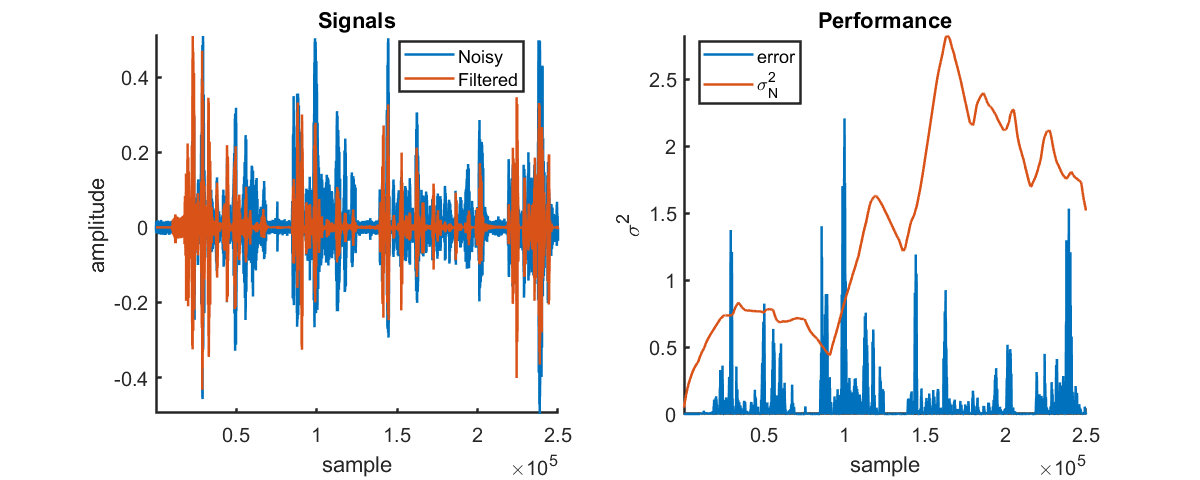
\includegraphics[width=\textwidth]{images/noisepsd.png}
  \caption{Results of the VAD based approach for estimating the noise PSD.}
  \label{fig:VADnoise}
\end{figure}

\subsection{Minimum Statistics Method}
The Minimum Statistics Method does not depend on the Voice Activity Detector and only depends on previous time frames of $y_{k}$ as can be seen in Equation \ref{eq:Q} and \ref{eq:Qmin}. Because using only the minimum value would be a underestimate of $E(|N|^2)$. A biasing factor, $B_{min}$ is added. This biasing factor used is the mean of the 10 previous values of $Q_k(l)$.
\begin{align}
Q_{k}(l) &= \alpha_k(l)Q_k(l-1)+(1-\alpha_k(l))\abs{y_{k}(l)}^{2}\label{eq:Qk} \\
  \mathbf{Q} &=
  \begin{Bmatrix}
    Q_{k}(l-L+1) & \hdots & Q_{k}(l)
  \end{Bmatrix}
  \label{eq:Q} \\
  \hat \sigma_{N,k}^{2}(l) &= B_{min}Q_{min}
  \label{eq:Qmin}\\
\end{align}

In Fig. \ref{fig:minstatnoise}, the results are shown. Here it shows that the noise is canceled very well. When more frames pass, the error increases in voiced areas. This could be due to the bias factor which was added or other mis-estimated variables. It seems to perform better than the VAD based approach in general. A big positive for this method is its independence.

\begin{figure}
  \centering
  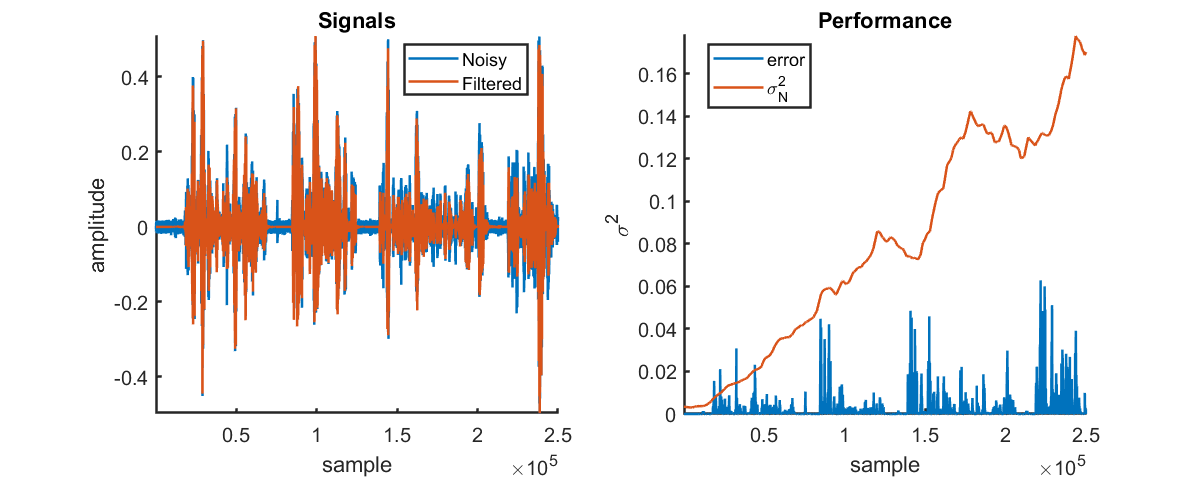
\includegraphics[width=\textwidth]{images/msmethod.png}
  \caption{Results of the Minimal Statistics based approach for estimating the noise PSD.}
  \label{fig:minstatnoise}
\end{figure}

\subsection{MMSE Method}
One of the more extensive methods discussed during the course is the MMSE Method. Equation \ref{eq:noiseMMSE1} looks similar to Equation \ref{eq:smoothingsigma} when speech is not present. Instead of using the PSD of the input signal $y_k(l)$, the noise its expected value is determined for that specific time-frame. This can be done as in Equation \ref{eq:noiseMMSE2}.
\begin{align}
  \widehat{\sigma_{N}^{2}}(l) &= \alpha \widehat{\sigma_{N}^{2}}(l-1) + (1-\alpha)E\left[ \abs{N_{k}(l)}^{2}\abs{y_{k}(l)}\right]
  \label{eq:noiseMMSE1} \\
  E\left[ \abs{N_{k}(l)}^{2}\abs{y_{k}(l)}\right] &=
  P\left(H_{0,k}(l)|y_{k}(l)\right) E\left[\abs{N_{k}(l)}^{2}\abs{y_{k}(l)},H_{0,k}\right] +
  P\left(H_{1,k}(l)|y_{k}(l)\right) E\left[\abs{N_{k}(l)}^{2}\abs{y_{k}(l)},H_{1,k}\right]
  \label{eq:noiseMMSE2}
\end{align}

There are some unknowns present. The change that speech is absent can be rewritten as in Equation \ref{eq:MMSEu1}. The expected values can be given as Formulas \ref{eq:MMSEu2} and \ref{eq:MMSEu3}.
\begin{align}
  P\left(H_{0,k}(l)|y_{k}(l)\right) &= 1 - P\left(H_{1,k}(l)|y_{k}(l)\right)
  \label{eq:MMSEu1} \\
  E\left[\abs{N_{k}(l)}^{2}\abs{y_{k}(l)},H_{0,k}\right] &= \abs{y_{k}(l)^{2}}
  \label{eq:MMSEu2} \\
  E\left[\abs{N_{k}(l)}^{2}\abs{y_{k}(l)},H_{1,k}\right] &= \widehat{\sigma_{N}^{2}}(l-1)
  \label{eq:MMSEu3}
\end{align}

This leaves only one function to be determined as which can be further broken down as in Equation \ref{eq:MMSEu4}. Of which the two elements are given by Equations \ref{eq:pyh0} and \ref{eq:pyh1}.
\begin{align}
  P\left(H_{1,k}(l)|y_{k}(l)\right) &= \frac{P\left(H_{1,k}(l))\right)p_{Y|H_{1}}}{P\left(H_{1,k}(l))\right)p_{Y|H_{1}} + P\left(H_{0,k}(l))\right)p_{Y|H_{0}}}
  \label{eq:MMSEu4}\\
  p_{Y|H_{0}} &= \frac{1}{\widehat{\sigma_{N}^{2}} \pi} \exp\left(-\frac{\abs{y^{2}}}{\widehat{\sigma_{N}^{2}}}\right)
  \label{eq:pyh0}\\
  p_{Y|H_{0}} &= \frac{1}{\widehat{\sigma_{N}^{2}} (1+\xi_{H_{1}})\pi} \exp\left(-\frac{\abs{y^{2}}}{\widehat{\sigma_{N}^{2}}(1+\xi_{H_{1}})}\right)
  \label{eq:pyh1}
\end{align}

However, $\xi_{H_{1}}$ is unknown and there is no sufficient a priori knowledge present to give an estimation of this variable. Which makes this method unfeasible to use.
